% !TEX root=main.tex

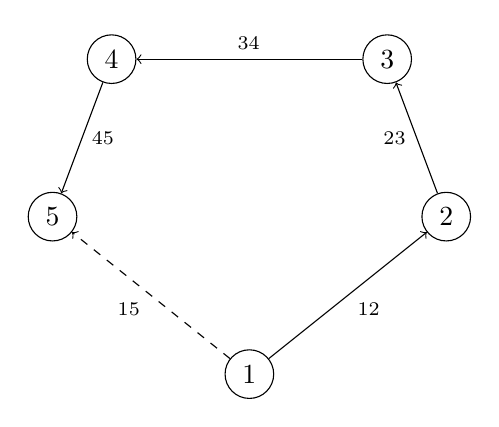
\begin{tikzpicture}
    \node[shape=circle,draw=black] (A) at (0,0) {$1$};
    \node[shape=circle,draw=black] (B) at (2.5,2) {$2$};
    \node[shape=circle,draw=black] (C) at (1.75,4) {$3$};
    \node[shape=circle,draw=black] (D) at (-1.75,4) {$4$};
    \node[shape=circle,draw=black] (E) at (-2.5,2) {$5$};

    \path [->] (A) edge node[right, yshift=-5pt] {$\eest_{12}$} (B);
    \path [->](B) edge node[left] {$\eest_{23}$} (C);
    \path [->](C) edge node[above] {$\eest_{34}$} (D);
    \path [->](D) edge node[right] {$\eest_{45}$} (E);
    \path [->](A) edge [dashed] node[left, yshift=-5pt] {$\eest_{15}$} (E);
\end{tikzpicture}
